\documentclass[12pt,english]{scrartcl}

\usepackage{amsmath,amsfonts,amssymb,amscd,amsthm,amsbsy,alltt,bera,upref,fancyvrb}
\usepackage[T1]{fontenc}
\usepackage{babel}
\usepackage{graphicx}
\usepackage{tikz}

\textheight=10.5truein
\textwidth=6.8truein
\hoffset=-.5truein
\voffset=-.5truein
\pagestyle{headings}
\footskip=36pt
\swapnumbers
\DefineVerbatimEnvironment{code}{Verbatim}{fontsize=\small}
\DefineVerbatimEnvironment{example}{Verbatim}{fontsize=\small}

\usepackage{xcolor}
\definecolor{shade}{RGB}{240,255,255}
\definecolor{nw}{RGB}{255,239,213}

\makeatletter
    \setkomafont{section}{\color{white}%
        \bfseries\Large
        
\begin{tikzpicture}[overlay]
        \draw[fill=black] (0,-2pt) rectangle
        (\linewidth,16.4pt);
        \end{tikzpicture}}
    \setkomafont{subsection}{\color{black}%
        \bfseries\Large
        \begin{tikzpicture}[overlay]
        \draw[fill=white] (0,-2pt) rectangle
        (\linewidth,16.4pt);
        \end{tikzpicture}}

\def\and{%
  \end{tabular}%
  \hskip 1em \@plus.10fil\relax
  \begin{tabular}[t]{c}}
\makeatother
\makeindex


\title{Technical Report: The Austinites}
\author{
  Sheeyla Garcia\\
  \and
  Jesus Hernandez\\
  \and
  Kyle Nicola\\
  \and
  Stephen Ridings\\
  \and
  Carlos Rodriguez\\
  \and
  Mark Sandan\\  
}
\date{ July 10, 2014 }
\begin{document}
\thispagestyle{plain}
\maketitle
\tableofcontents

\begin{figure}[h!]
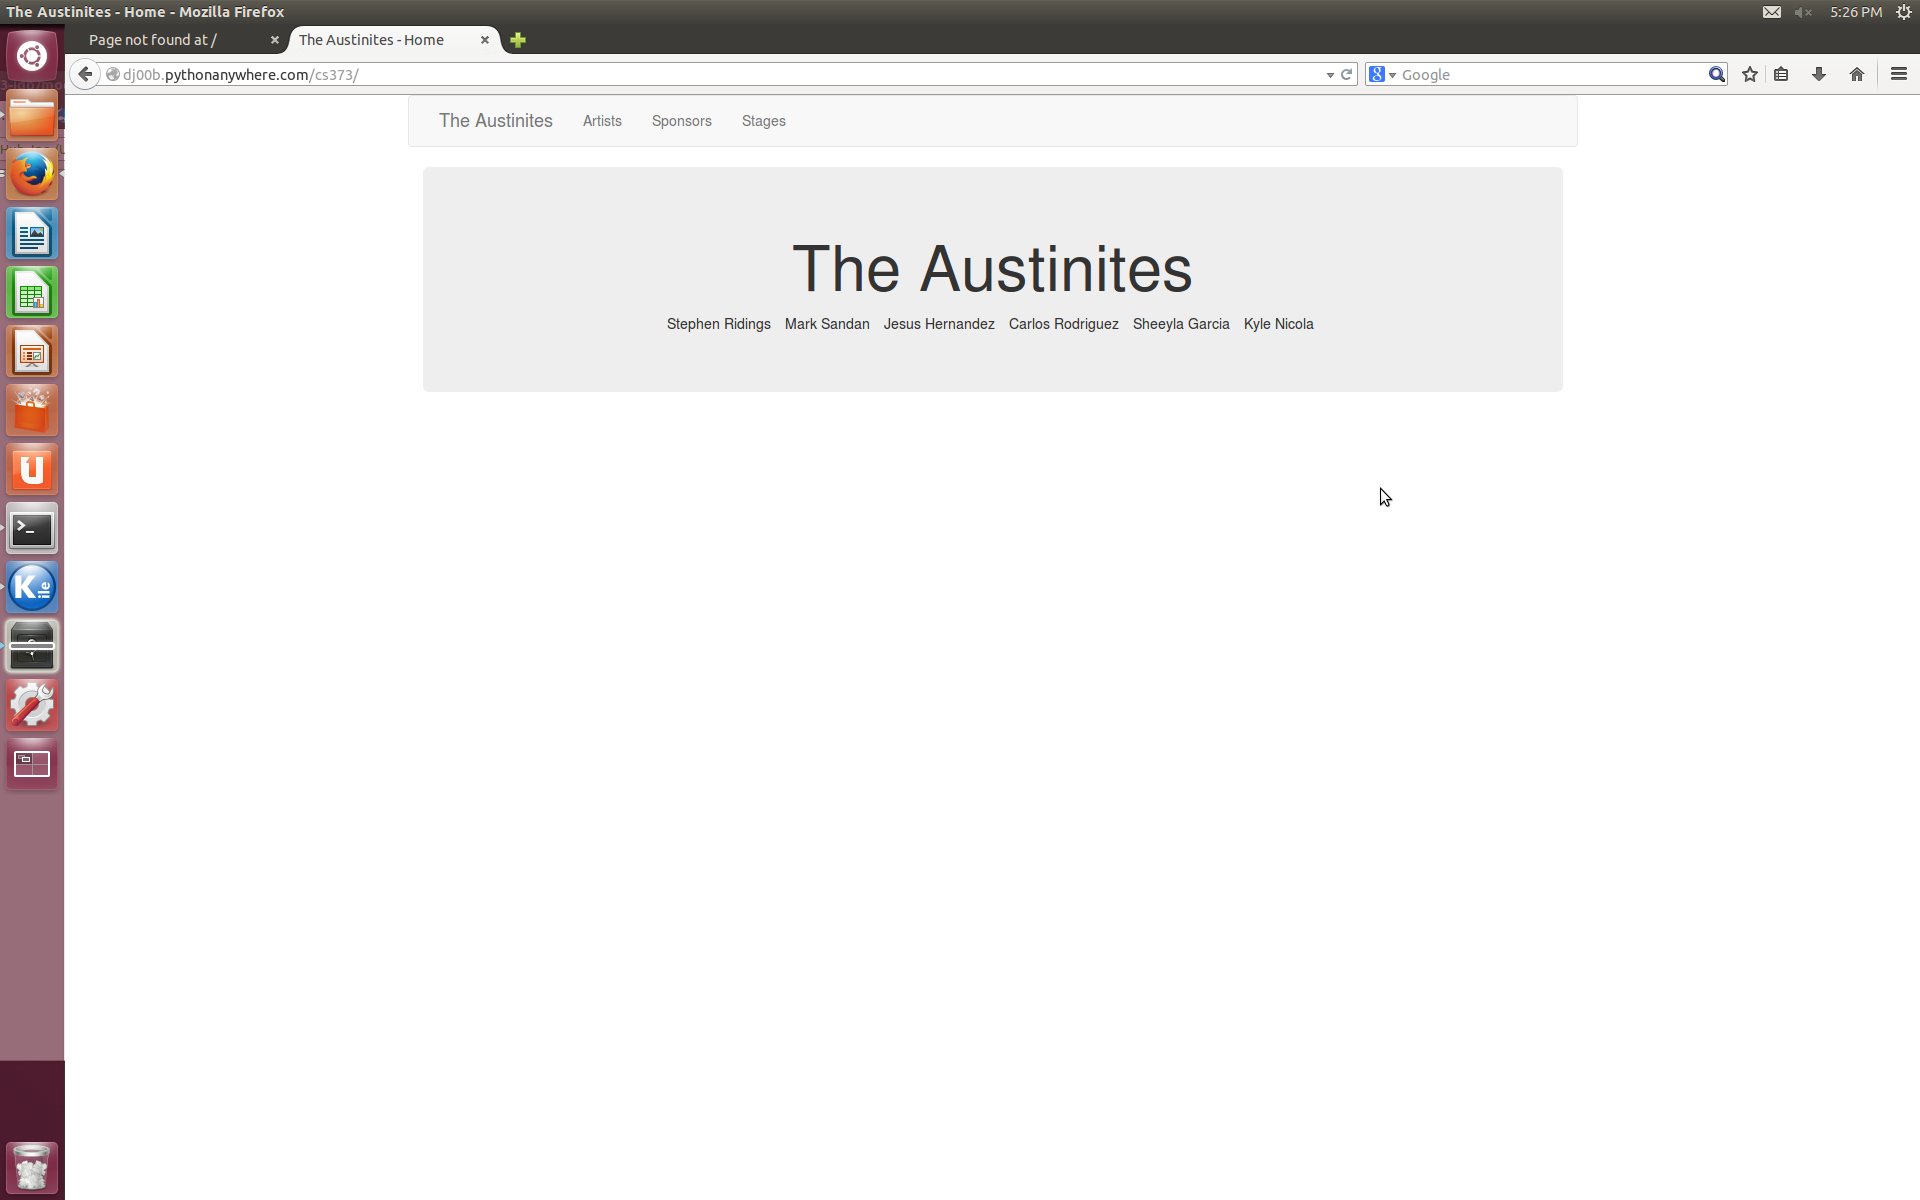
\includegraphics[width=\textwidth]{home}
 \caption{Example Home page showing the group name and the links to the three main pages.}
\end{figure}

\section{Introduction}
The website we are designing is about the 2014 Austin City Limits (ACL) music festival. The website design has three main pages: Artists, Stages, and Sponsors.
The website allows anyone to view pages about current Artists, Sponsors, and Stages.

The technologies used are PythonAnywhere, Python 3.4, Django 1.6,
Twitter Bootstrap 3.2, Apiary, and the database sqlite3. PythonAnywhere is used to host the site using the Django web-framework to 
construct the necessary models and views to handle HTTP requests. Twitter Bootstrap is used to organize common data among different
types of pages into a base template HTML file. 

A problem that we are facing is that the information we need to complete the project hasn't been published as of the dat this report
is being written. Currently we are using stubbed relationships to 

\section{Design}
Our current design of the website uses HTML and Twitter Bootstrap to stylize each page and PythonAnywhere to host the page. 
Using Django's templating language we are able to reuse html files by extending from them. Currently we only have a single base html page that
uses Twitter Bootstrap. We have nine pages in static HTML that provide examples of the web page design and content.


\begin{figure}[h!]
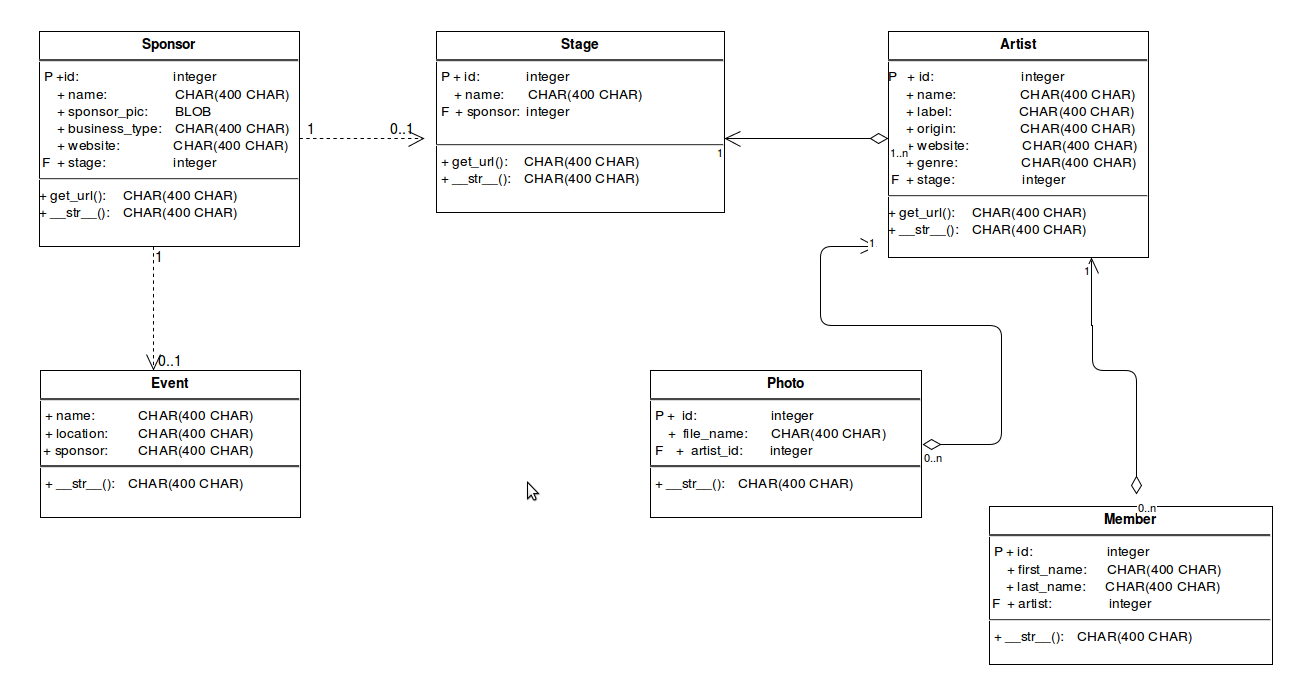
\includegraphics[width=\textwidth]{UML}
 \caption{The current UML schema depicting the relationships between the Django models.}
\end{figure}

\subsection{Web Pages}
Each web page has basic information about a particular artist, sponsor, or stage involved in the ACL music festival.
Each page includes a bio, video, official website, Youtube channel, a Twitter feed, and Picture.
\subsubsection{Artists}
Artist Pages can be reached from the home page or from Stage pages depending on whether the Artist played on
a Stage that was hosted by a Sponsor. 
\subsubsection{Sponsors}
Sponsor pages can be reached from the home page or from 

\subsubsection{Stages}


\subsection{RESTful  API}
The API allows GET requests to the following models: Stages, Sponsors, Artists, Members, and  Photos.
The following section will detail the attributes for the modules, and how the server will respond to the GET requests.
\subsubsection{Stages}
When a GET is called on $[/stages]$ it will return a HAL+JSON representation all the Stages in the database.  It will be a list of the stages along with their attributes.
When a GET is called on $[/stages/{id}]$ it will return a HAL+JSON representation of a single Stage in the database with the given id.  It will list the stage and all of it's attributes
Example of single stage:
\begin{verbatim}
{
         "_links": {
                "self": { "href": "stages/42" }
         },
         "id": 42,
         "name": "Stage name"
}
\end{verbatim}
\subsubsection{Sponsor}
When a GET is called on $[/sponsors]$ it will return a HAL+JSON representation all the Sponsors in the database.  It will be a list of the sponsors along with their attributes.
When a GET is called on $[/sponsors/{id}]$ it will return a HAL+JSON representation of a single Sponsor in the database with the given id.  It will list the sponsor and all of it's attributes
Example of single sponsor:
\begin{verbatim}
{
        "_links": {
                "self": { "href": "sponsors/42" }
        },
        "id": 42,
        "name": "Sponsor name",
        "business_type": "Type of Business",
        "website": "URL of sponsor website",
        "stage": 12
}
\end{verbatim}

\subsubsection{Artist}
When a GET is called on $[/artists]$ it will return a HAL+JSON representation all the Artists in the database.  It will be a list of the artists along with their attributes.
When a GET is called on $[/artists/{id}]$ it will return a HAL+JSON representation of a single Artist in the database with the given id.  It will list the artist and all of it's attributes

Example of single artist:
\begin{verbatim}
{
        "_links": {
               "self": { "href": "artists/42" }
        },
        "id": 42,
        "name": "Artist name"
        "label": "Label of artist"
        "origin": "Where the artist was from"
        "website": "URL to the artist"
        "genre": "Genre of the artist"
        "stage": 22
}
\end{verbatim}
\subsubsection{Member}
When a GET is called on $[/artists/{artist\_id}/members/]$ it will return a HAL+JSON representation all the Members in the database for the given artist id.  It will be a list of the members along with their attributes.
When a GET is called on $[/artists/{artist\_id}/members/{id}]$ it will return a HAL+JSON representation of a single Member in the database with the given id.  It will list the member and all of it's attributes

Example of single member:
\begin{verbatim}
{
        "_links": {
               "self": { "href": "artists/22/members/42" }
        },
        "id": 42,
        "first_name": "Member's first name"
        "last_name": "Member's last name"
        "artist_id": 22
}
\end{verbatim}
\subsubsection{Photo}
When a GET is called on $[/artists/{artist\_id}/photos/]$ it will return a HAL+JSON representation all the Photos in the database for the given artist id.  It will be a list of the photos along with their attributes.
When a GET is called on $[/artists/{artist\_id}/photos/{id}]$ it will return a HAL+JSON representation of a single Photo in the database with the given id.  It will list the photo and all of it's attributes

Example of single photo:
\begin{verbatim}
{
        "_links": {
               "self": { "href": "artists/22/photos/42" }
        },
        "id": 42,
        "file_name": "photo.jpg"
        "artist_id": 22
}
\end{verbatim}

\subsection{Django Models}
The Django models created represent the entities we intend to keep in the database for the future when use dynamically loaded pages.
The following subsections document the attributes and intended functionality of each class instance method. 
\subsubsection{Artist}
The Artist class represents the current Artists playing on a sponsored stage. All Artists will be a child of some
stage depending on whether they are playing that Stage or not. We are assuming that an Artist will play on 
exactly one stage. The Artist class is implemented using the following:
\begin{verbatim}
attributes:
- id: Primary Key, integer type field.
- name: the name of max length 400 characters.
- label: the artist label with a maximum length of 400 characters.
- origin: the place of origin the artist/group formed with a maximum length of 400 characters.
- website: the official website of the artist or fan site if none. Maximum length of 400 characters.
- genre: the genre associated with the artist. May span more than one. maximum length of 400 characters.
- stage: Foreign Key, integer of type field.

methods:
- get.url(): returns the string "/artists/{id}" . Maximum of number of 400 characters.
- __str__(): returns the name string of the artist.
\end{verbatim}


\subsubsection{Sponsor}
The Sponsor class represents the ACL sponsors that sponsor a Stage for the Artist to perform on.
This relationship is expressed using the one-to-many relationship between the Sponsor and the Stage
class. 

The Sponsor class has the following attributes and methods:
\begin{verbatim}
attributes:
- id: Primary Key, integer type field
- name: a character type field with a maximum length of 400 characters
- business_type: a character type field with a maximum length of 400 characters
- website: a character type field with a maximum length of 400 characters
- stage: Foreign Key, integer of type field

methods:
- get.url(): returns the string "/sponsors/{id}". Maximum number of 400 characters.
- __str__(): returns a string that represents the name of the sponsor.
\end{verbatim}

\subsubsection{Stage}
The Stage class is meant to represent the stage that an Artist will perform on. All stages
have one sponsor. The Stage class extends from the Django models.Models class.

The Stage class has the following attributes and methods:
\begin{verbatim}
attributes:
- id: Primary Key, integer type field
- name: a character type field with a maximum length of 400 characters
- sponsor: Foreign Key, integer of type field

methods:
- get.url(): returns the string "/stages/%s/{name}" where name is the stage name.
- __str__(): returns a string that represents the name of the stage
\end{verbatim}

\subsubsection{Photo}
The Photo class represents a path to a photo of an Artist. 
All Photo's are associated with an Artist in a many-to-one relationship.
This is expressed with the Foreign key being an Artist that the Photo is associated with. 
The Photo class has the following attributes and methods:
\begin{verbatim}
attributes:
-file_name: A CharField of 400 characters. File name of the photo. 
-artist: The ForeignKey relating a Photo to an Artist.

methods:
- __str__(): returns the file_name of the photo.
\end{verbatim}

\subsubsection{Member}
The Member class is meant to represent the members of the Artist group. The Member class has the following attributes and methods:
\begin{verbatim}
attributes:
-first_name: A CharField of 400 characters. 
-last_name: A CharField of 400 characters.
-artist: ForeignKey relating the Member to Artist. Integer type field.

methods:
- __str__(): returns the string of form "{first_name} {last_name}" if there is
             a last anme available. Otherwise "{first_name}" is returned.
\end{verbatim}

\section{Unit Tests}

\section{Expansions}
In future releases our website will include an SQLite database. This database will store all information regarding the models and will interact as documented in the RESTful API section.
In turn, our HTML pages will utilize this database to work dynamically, as opposed to the static pages currently implemented.
We also plan to display more information in the HTML pages.
For example, artist pages will include information on members or link to more social media accounts, such as Instagram or SoundCloud.
Stage pages will also link to a map of the festival so users can see their location.
The Django models will also grow. All models will include a set method in addtition to the get method that is already provided.
The Sponsor model will also include a sponsor_pic attribute for its logo. 
Sponsor models might also include include an attribute to store the location of their headquarters or the name of their respective CEOs.
Optionally, Member models might also include an attribute to store the insturment(s) the member plays.
In response to the growth of the models the unit tests will become more robust.
These tests will will check that the database is correctly populated with its new attributes as well as test all the new methods included.
In addition to the growth of the models, the API will also grow to accomodate. The updated API will include the option to make put requests or delete requests.

\end{document}
